\documentclass[10pt,a4paper]{amsart}
\usepackage[margin=19mm]{geometry}
\usepackage{amsmath,amssymb,mathtools}
\usepackage[scr=rsfs,cal=euler]{mathalfa}
\usepackage{xfrac}
\usepackage[unicode,hidelinks,bookmarks=false]{hyperref}
\newcommand{\ie}{i.e.\ }
\newcommand{\cf}{cf.\ }
\newcommand{\resp}{respectively\ }
\newcommand{\Subsection}{\subsection}
\providecommand{\nobreakdash}{\nobreak\hbox{-}}
\setlength{\emergencystretch}{2em}
\multlinegap0pt
\usepackage{tikz}
\usepackage{amssymb}
\usepackage{siunitx}
\newtheorem{theorem}{Theorem}
\newcommand{\abs}[1]{\left|#1\right|}
\newcommand{\ka}{k_{\mathrm{a}}}
\DeclareMathOperator*{\leng}{length}
\newcommand{\mx}{\mathbf{x}}
\newcommand{\mz}{\mathbf{z}}
\newcommand{\p}{\partial}
\newcommand{\rd}{\mathrm{d}}
\DeclareMathOperator*{\reg}{reg}
\DeclareMathOperator*{\sing}{sing}
\newcommand{\vn}{\boldsymbol{\nu}}
\newcommand{\vt}{\boldsymbol{\theta}}
\title{Topological derivative for a fast identification of short, linear perfectly conducting cracks with inaccurate background information}
\author{Won-Kwang Park}
\date{Source: arXiv:2504.19485v1 (CC BY 4.0)}
\begin{document}
\maketitle

\noindent\emph{Source and licence.} Topological derivative for a fast identification of short, linear perfectly conducting cracks with inaccurate background information. Version arXiv:2504.19485v1 (CC BY 4.0), distributed by arXiv under the Creative Commons Attribution 4.0 International licence, http://creativecommons.org/licenses/by/4.0/, as recorded in the arXiv licence metadata for this exact version and shown on the abstract page https://arxiv.org/abs/2504.19485v1. Full licence notice: \texttt{licenses/arxiv-2504.19485-CC-BY-4.0.txt}.\par\smallskip

\noindent\textit{Editorial scope.} Counted unit: the article's theorem Theorem (source0.tex lines 205--211). The article's complete original proof of it is delivered with it (source0.tex lines 212--261, one \texttt{proof} environment of 50 lines). No mathematics is written, repaired or re-derived: the statement and the proof are the article's own lines, in the article's own notation, and no retained line is substituted or re-flowed.  Retained uncounted as the source-local context the proof needs: lines 176--178; lines 180--185; lines 193--195; lines 263--285.  Nothing was omitted from any retained span, so the package carries no omission record.  The retained lines cite 2 works, whose entries are transcribed verbatim from the article's own bibliography source in the e-print and delivered with short editorial labels recorded in the item's reference mapping.  The retained lines contain the article's own diagram code, which the wrapper typesets with the standard tikz packages; no image file is delivered and the package declares no asset dependency.  Editorial formatting only, in addition: an AMS \texttt{amsart} preamble that restates the article's own declarations and macros used by the retained lines, namely the environments \texttt{theorem} on separate counters, together with the standard packages those lines need.  The retained environments print in this document as Theorem 1 in order of appearance, whereas the article prints the same items with the numbering of its own full document.  The complete native source of the article as distributed in the arXiv e-print for this exact version is bundled unchanged as \texttt{sources/177182/source0.tex}.
\begin{equation}\label{NormalizedTopologicalDerivative}
  \mathfrak{F}(\mz;\ka)=\frac{|d_T\mathbb{E}(\mz;\ka)|}{\displaystyle\max_{\mz\in\Omega}|d_T\mathbb{E}(\mz;\ka)|}\quad\text{where}\quad d_T\mathbb{E}(\mz;\ka)=\mathrm{Re}\sum_{n=1}^{N}v^{(n)}(\mz;\ka)\overline{w^{(n)}(\mz;\ka)},
\end{equation}

\begin{equation}\label{Adjoint2}
  \left\{\begin{array}{rcl}
    \displaystyle\Delta v^{(n)}(\mx;\ka)+\ka^2 v^{(n)}(\mx;\ka)=0&\mbox{in}&\Omega\\
\noalign{\medskip}\displaystyle\frac{\p v^{(n)}(\mx;\ka)}{\p\vn(\mx)}=u^{(n)}(\mx;k)-w^{(n)}(\mx;k)&\mbox{on}&\p\Omega.
  \end{array}\right.
\end{equation}

\begin{equation}\label{Asymptoticformula}
u^{(n)}(\mx;k)-w^{(n)}(\mx;k)=\sum_{m=1}^{M}\frac{2\pi}{\ln(\ell_m/2)}w^{(n)}(\mx_m;k)\mathcal{N}(\mx,\mx_m;k)+\mathcal{O}\left(\frac{1}{|\ln\ell_m|^2}\right),
\end{equation}

\begin{figure}[h]
\begin{center}
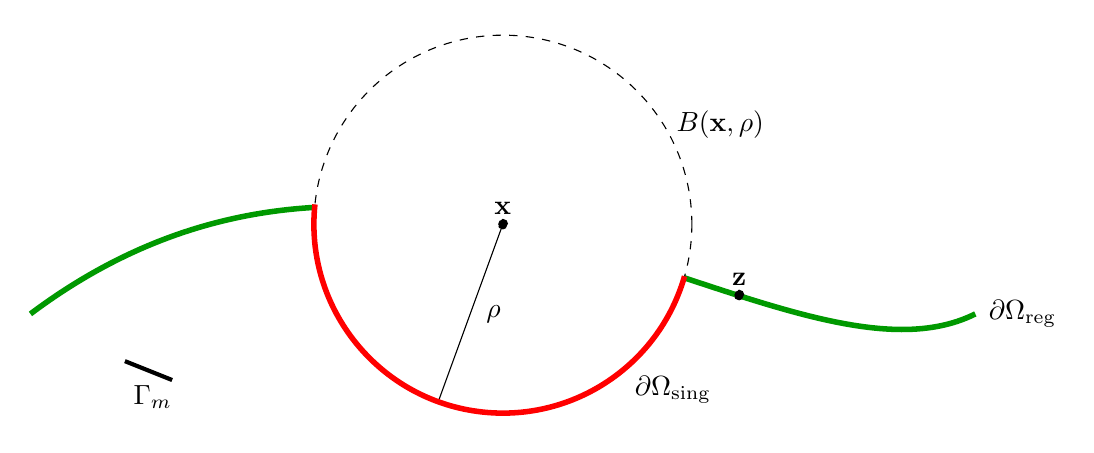
\begin{tikzpicture}[scale=1.2]
\def\SA{174};
\def\FA{344};
\draw[green!60!black,rounded corners,line width=2pt,fill=white] (-5,0) .. controls (-1,3) and (3,-1) .. (5,0);
\node at (5.5,0) {$\p\Omega_{\reg}$};
\draw[fill=white,dashed] (0,0.95) circle [radius=2];
\node at (2.3,2) {$B(\mx,\rho)$};
\draw[black,-] (0,0.95) -- ({2*cos(250)},{2*sin(250)+0.95});
\node at (-0.1,0) {$\rho$};
\draw[red,solid,line width=2pt] ({2*cos(\SA)},{2*sin(\SA)+0.95}) arc (\SA:\FA:2);
\node at (1.8,-0.8) {$\p\Omega_{\sing}$};
\draw[fill=black,dashed] (0,0.95) circle [radius=0.05];
\node [above] at (0,0.95) {$\mx$};
\draw[fill=black,dashed] (2.5,0.2) circle [radius=0.05];
\node [above] at (2.5,0.2) {$\mz$};
\draw[black,line width=1.5pt,-] (-4,-0.5) -- (-3.5,-0.7) node [below,xshift=-7,yshift=2] {$\Gamma_m$};
\end{tikzpicture}
\caption{\label{Boundaries}Illustration of $\p\Omega_{\sing}$ and $\p\Omega_{\reg}$.}
\end{center}
%\draw[rounded corners,thick] (-5,0) .. controls (-4,1.5) and (-2,2) .. (-1.75,0.95);
\end{figure}

\begin{theorem}\label{Theorem}
For sufficiently large $N$, $\mathfrak{F}(\mz;\ka)$ can be represented as follows
\begin{equation}\label{Structure_Function}
\mathfrak{F}(\mz;\ka)\approx\frac{|\Phi(\mz)|}{\displaystyle\max_{\mz\in\Omega}|\Phi(\mz)|},\quad\Phi(\mz)=\sum_{m=1}^{M}\frac{J_0(|k\mx_m-\ka\mz|)}{\ln(\ell_m/2)},
\end{equation}
where $J_0$ is the Bessel function of order zero of the first kind.
\end{theorem}

\begin{proof}
Since $v^{(n)}(\mx;\ka)$ satisfies \eqref{Adjoint2}, for $\mz\in\Omega\backslash\p\Omega$, we have
\begin{equation}\label{FormulaV}
v^{(n)}(\mz;\ka)=\int_{\p\Omega}\frac{v^{(n)}(\mx;\ka)}{\p\vn(\mx)}\mathcal{N}(\mx,\mz;\ka)\rd\mx=\int_{\p\Omega}\left(u^{(n)}(\mx;k)-w^{(n)}(\mx;k)\right)\mathcal{N}(\mx,\mz;\ka)\rd\mx.
\end{equation}
Applying \eqref{Asymptoticformula} and \eqref{FormulaV} to \eqref{NormalizedTopologicalDerivative}, we can obtain
\begin{align}
\begin{aligned}\label{Term}
d_T\mathbb{E}(\mz;\ka)&=\mathrm{Re}\sum_{n=1}^{N}v^{(n)}(\mz;\ka)\overline{w^{(n)}(\mz)}\\
&\approx\mathfrak{Re}\sum_{n=1}^{N}\left[\int_{\p\Omega}\left(u^{(n)}(\mx;k)-w^{(n)}(\mx)\right)\mathcal{N}(\mx,\mz;\ka)\rd\mx\right]\overline{w^{(n)}(\mz;\ka)}\\
&\approx\mathfrak{Re}\sum_{n=1}^{N}\left[\int_{\p\Omega}\left(\sum_{m=1}^{M}\frac{2\pi}{\ln(\ell_m/2)}w^{(n)}(\mx_m;k)\mathcal{N}(\mx,\mx_m;k)\right)\mathcal{N}(\mx,\mz;\ka)\rd\mx\right]\overline{w^{(n)}(\mz;\ka)}\\
&=\mathfrak{Re}\sum_{m=1}^{M}\frac{2\pi}{\ln(\ell_m/2)}\left(\int_{\p\Omega}\mathcal{N}(\mx,\mx_m;k)\mathcal{N}(\mx,\mz;\ka)\rd\mx\right)\left(\sum_{n=1}^{N}w^{(n)}(\mx_m;k)\overline{w^{(n)}(\mz;\ka)}\right).
\end{aligned}
\end{align}

Since the following relationship holds for sufficiently large $N$ (see \cite{P-SUB3} for derivation),
\[\frac{1}{N}\sum_{n=1}^{N}\exp(\vt_n\cdot\mx)\approx J_0(|\mx|),\]
we can derive
\begin{equation}\label{Term1}
\sum_{n=1}^{N}w^{(n)}(\mx_m;k)\overline{w^{(n)}(\mz;\ka)}=\sum_{n=1}^{N}\exp\Big(\vt_n\cdot(k\mx_m-\ka\mz)\Big)=NJ_0(|k\mx_m-\ka\mz|).
\end{equation}

Next, following to \cite{AKL}, the Neumann function $\mathcal{N}$ has a logarithmic singularity. Thus, it can be decomposed into the singular and regular functions;
\[\mathcal{N}(\mx,\mz;k)=-\frac{1}{2\pi}\ln|\mx-\mz|+\mathcal{R}(\mx,\mz;k),\quad\mx\ne\mz,\]
where $\mathcal{R}(\mx,\mz;k)\in\mathcal{C}^{1,\alpha}$ in both $\mathbf{x}$ and $\mathbf{y}$ for some $\alpha$ with $0<\alpha<1$. Since $\mx\in\p\Omega$ and $\mx_m\in\Gamma_m$, there is no blow up of $\mathcal{N}(\mx,\mx_m;k)$ so that
\[|\mathcal{N}(\mx,\mx_m;k)|\leq\frac{1}{2\pi}\ln|\mx-\mx_m|+|\mathcal{R}(\mx,\mx_m;k)| <\frac{1}{2\pi}\ln\mbox{diam}(\Omega)+\max_{\mx\in\p\Omega}|\mathcal{R}(\mx,\mx_m;k)|,\]
where $\mbox{diam}(\Omega)$ denotes the diameter of $\Omega$. Hence, applying H{\"o}lder's inequality yields
\[\abs{\int_{\p\Omega}\mathcal{N}(\mx,\mx_m;k)\mathcal{N}(\mx,\mz;\ka)\rd\mx}\leq \bigg(\frac{1}{2\pi}\ln\mbox{diam}(\Omega)+\max_{\mx\in\p\Omega}|\mathcal{R}(\mx,\mx_m;k)|\bigg) \int_{\p\Omega}|\mathcal{N}(\mx,\mz;\ka)|\rd\mx.\]
Now, we consider the singularity of $\mathcal{N}(\mx,\mz;\ka)$ when $\mz\in\Omega$ is close to $\mx\in\p\Omega$. To this end, for sufficiently small constant $\rho>0$, generate a ball $B(\mx,\rho)$ with radius $\rho$ and center $\mx$ such that
\[B(\mx,\rho)\cap\Gamma=\varnothing.\]
Based on this, let us split $\p\Omega$ into two smooth curves $\p\Omega=\p\Omega_{\sing}\cup\p\Omega_{\reg}$ (see Figure \ref{Boundaries} for illustration), where
\[\p\Omega_{\sing}=\Omega\cap\p B(\mx,\rho)\quad\text{and}\quad\p\Omega_{\reg}=\p\Omega\backslash\overline{\p\Omega_{\sing}}.\]
Then, we can examine that
\begin{align*}
\int_{\p\Omega}|\mathcal{N}(\mx,\mz;\ka)|\rd\mx\leq &\frac{1}{2\pi}\int_{\p\Omega}\ln|\mx-\mz|\rd\mx +\int_{\p\Omega}|\mathcal{R}(\mathbf{z},\mathbf{y};\omega)|\rd\mx\\
\leq&\frac{1}{2\pi}\lim_{\rho\to0+}\left(\int_{\p\Omega_S}\ln|\mx-\mz|\rd\mx +\int_{\p\Omega_R}\ln|\mx-\mz|\rd\mx\right)+\max_{\mx\in\p\Omega}|\mathcal{R}(\mx,\mz;\ka)|\leng(\p\Omega)\\
\leq&\frac{1}{2\pi}\lim_{\rho\to0+}\bigg(\rho\ln\rho+(\leng(\p\Omega)-\rho)\ln|\leng(\p\Omega)|\bigg)+\max_{\mx\in\p\Omega}|\mathcal{R}(\mx,\mz;\ka)|\leng(\p\Omega)\\
=&\leng(\p\Omega)\bigg(\frac{1}{2\pi}\ln|\leng(\p\Omega)|+\max_{\mx\in\p\Omega}|\mathcal{R}(\mx,\mz;\ka)|\bigg).
\end{align*}
Here, $\leng(\p\Omega)$ denotes the length of $\partial\Omega$. Therefore,
\begin{multline}\label{Term2}
  \abs{\int_{\p\Omega}\mathcal{N}(\mx,\mx_m;k)\mathcal{N}(\mx,\mz;\ka)\rd\mx}\leq\bigg(\frac{1}{2\pi}\ln\mbox{diam}(\Omega)+\max_{\mx\in\p\Omega}|\mathcal{R}(\mx,\mx_m;k)|\bigg) \times\\
  \leng(\p\Omega)\bigg(\frac{1}{2\pi}\ln|\leng(\p\Omega)|+\max_{\mx\in\p\Omega}|\mathcal{R}(\mx,\mz;\ka)|\bigg).
\end{multline}
This means that there is no blowup of $\int_{\p\Omega}\mathcal{N}(\mx,\mx_m;k)\mathcal{N}(\mx,\mz;\ka)\rd\mx$ for any $\mx\in\p\Omega$ and $\mz\in\Omega$.

Plugging \eqref{Term1} and \eqref{Term2} into \eqref{Term}, we can examine that
\[d_T\mathbb{E}(\mz;\ka)\propto\sum_{m=1}^{M}\frac{J_0(|k\mx_m-\ka\mz|)}{\ln(\ell_m/2)}\]
and correspondingly, \eqref{Structure_Function} can be ontained.
\end{proof}

\begin{thebibliography}{99}
\bibitem[AKL]{AKL} \newblock H.~Ammari, H.~Kang and H.~Lee, \newblock \emph{Layer Potential Techniques in Spectral Analysis}, vol. 153 of Mathematical surveys and monographs, \newblock American Mathematical Society, 2009.
\bibitem[P-SUB3]{P-SUB3} \newblock W.-K. Park, \newblock Multi-frequency subspace migration for imaging of perfectly conducting, arc-like cracks in full- and limited-view inverse scattering problems, \newblock \emph{J. Comput. Phys.}, \textbf{283} (2015), 52--80.
\end{thebibliography}
\end{document}
